\section{Results}
\label{sec:results}

\begin{figure}[ht]
\centering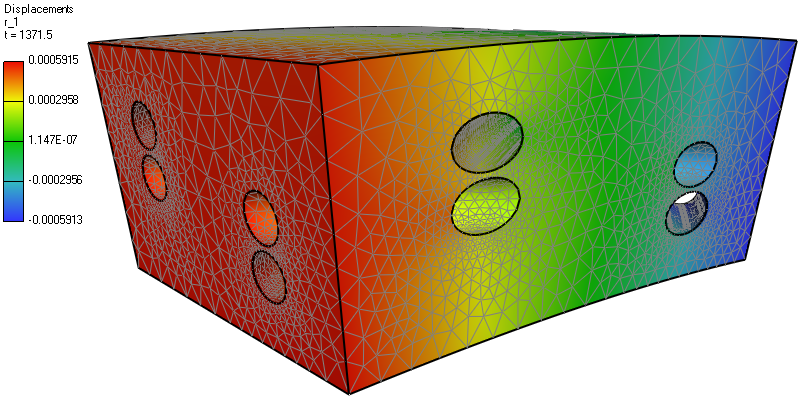
\includegraphics[width=\textwidth]{figures/temelin_screenshot}
\caption{Temelin nuclear power plant. Results visualization (Displacement field, X component).}
\label{fig:temelin:mesh}
\end{figure}

\begin{figure}[ht]
\centering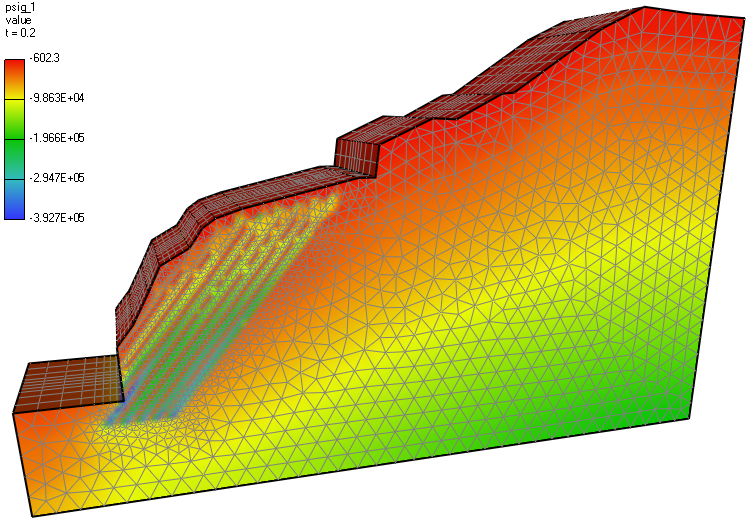
\includegraphics[width=\textwidth]{figures/chotkova_screenshot}
\caption{Chotkova geologic layers. Results visualization (Stress field, sigma XX component).}
\label{fig:chotkova:mesh}
\end{figure}

\begin{figure}[ht]
\centering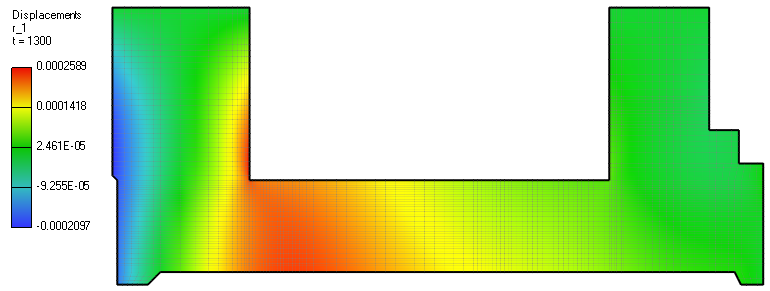
\includegraphics[width=\textwidth]{figures/mechaxisym_screenshot}
\caption{"Mechaxisym" model. Results visualization (Displacement field, X component).}
\label{fig:mechaxisym:mesh}
\end{figure}

\begin{figure}[ht]
\centering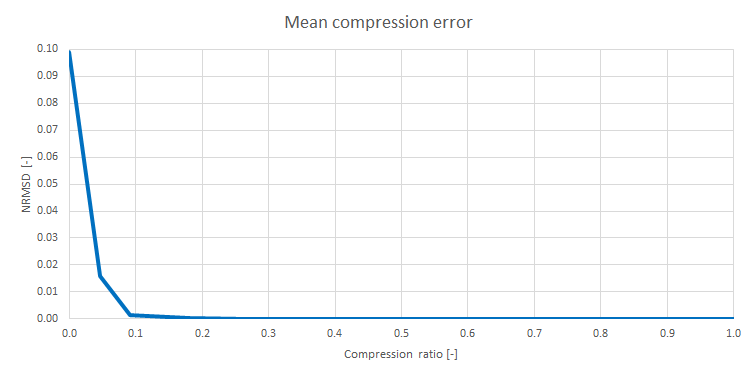
\includegraphics[width=\textwidth]{figures/chotkova_NRMSD}
\caption{Dependence of Normalized Rooted Mean Squared Deviation on Compression ratio for Chotkova project results.}
\label{fig:chotkova:NRMSD}
\end{figure}

\begin{figure}[ht]
\centering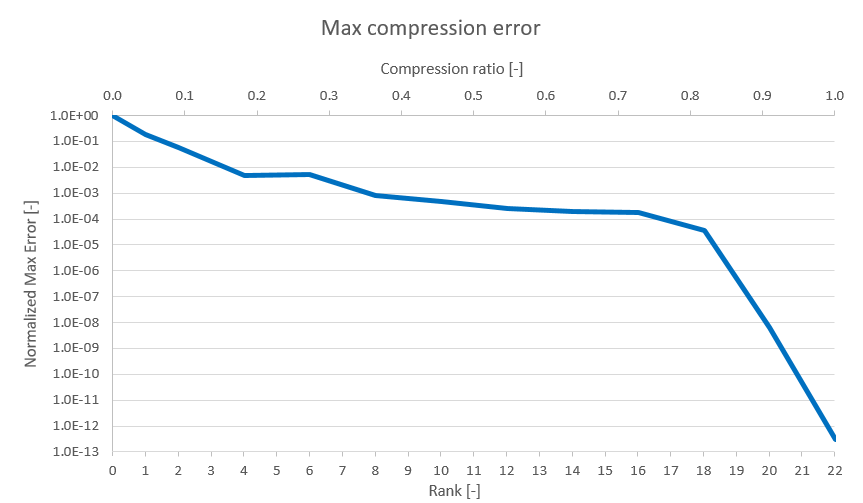
\includegraphics[width=\textwidth]{figures/chotkova_MaxError}
\caption{Dependence of Normalized Max Error on Compression ratio for Chotkova project results.}
\label{fig:chotkova:MaxError}
\end{figure}

\begin{figure}[ht]
\centering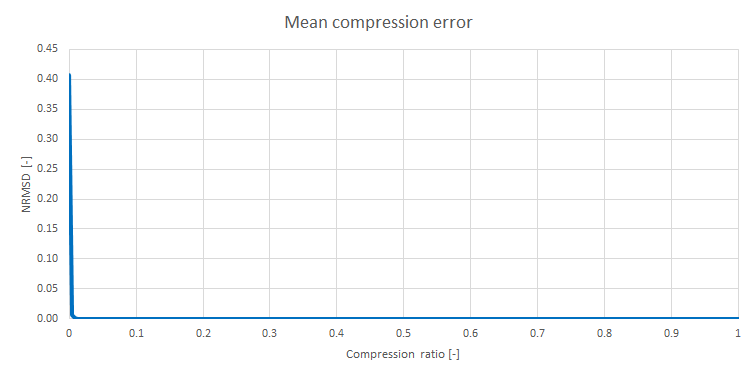
\includegraphics[width=\textwidth]{figures/mechaxisym_NRMSD}
\caption{Dependence of Normalized Rooted Mean Squared Deviation on Compression ratio for Mechaxisym project results.}
\label{fig:mechaxisym:NRMSD}
\end{figure}

\begin{figure}[ht]
\centering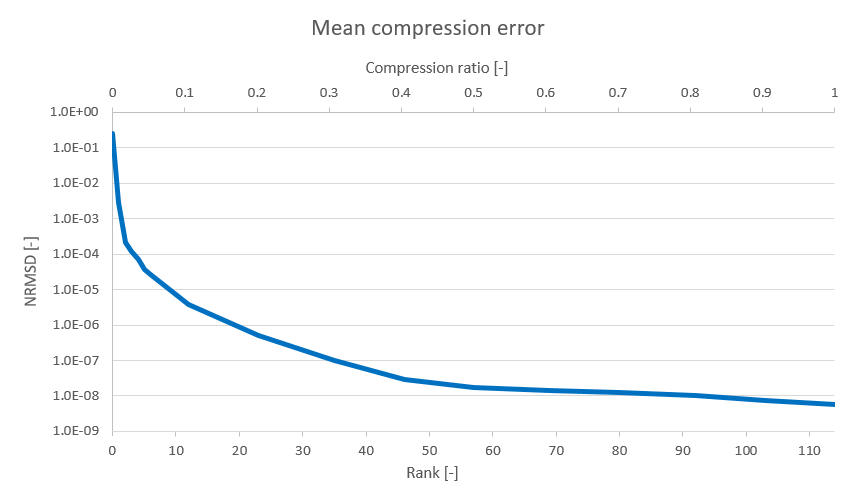
\includegraphics[width=\textwidth]{figures/temelin_NRMSD}
\caption{Dependence of Normalized Rooted Mean Squared Deviation on Compression ratio for Temelin project results.}
\label{fig:temelin:NRMSD}
\end{figure}

\begin{figure}[ht]
\centering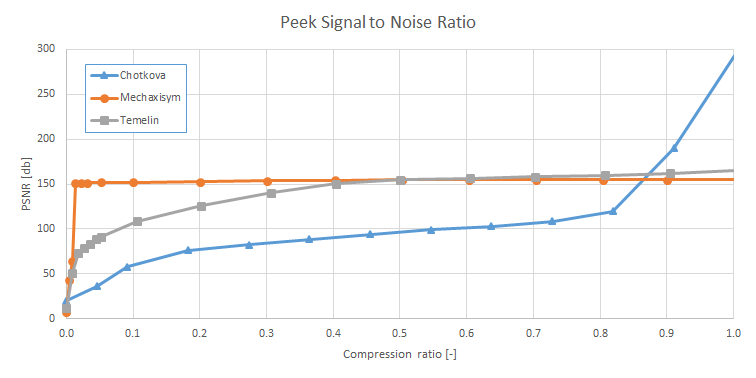
\includegraphics[width=\textwidth]{figures/PSNR}
\caption{Comparison of Peek signal to noise ratio value calculated for different decompositions.}
\label{fig:PSNR}
\end{figure}

\begin{figure}[ht]
\centering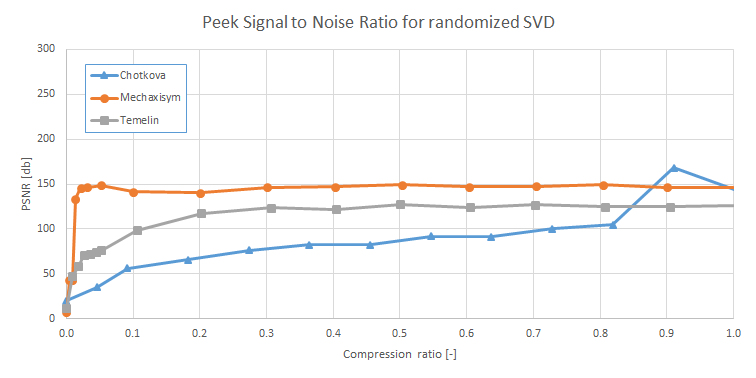
\includegraphics[width=\textwidth]{figures/PSNR_rand}
\caption{Comparison of Peek signal to noise ratio value for different randomized decompositions.}
\label{fig:PSNR_rand}
\end{figure}

\begin{figure}[ht]
\centering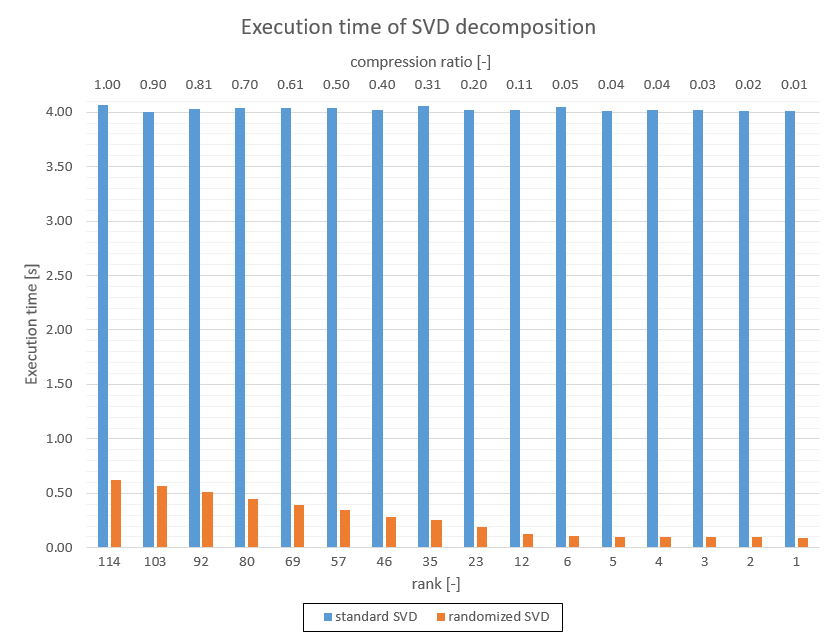
\includegraphics[width=\textwidth]{figures/temelin_ExecutionTime}
\caption{Variation of execution time of standard and randomized decompositions calculated for Temelin project results. Execution time of standard SVD is independent of target rank whereas execution time of randomized SVD decreases linearly with increasing target rank.}
\label{fig:temelin:ExeTime}
\end{figure}
